% SPDX-License-Identifier: CC-BY-4.0
%
% results.tex - Report the findings of the research.
%
% Present observations, measurements, or outcomes in a clear order before
% interpreting their meaning in the analysis section.

\subsection{Diagrama de clases}

La \infig{fig:diagrama-clases} reconstruye el diagrama de clases de la aplicación con las tres familias de patrones, en una página horizontal para que se pueda leer. Las clases se agrupan en sus paquetes, y el color del encabezado indica el patrón al que pertenecen: morado para Command, morado oscuro para Observer, naranja para Iterator y lila para los patrones de la actividad anterior. Las clases que el diseño cambia muestran sus atributos y métodos, y las que quedan como en la actividad anterior se muestran solo con su nombre.

\begin{landscape}
\begin{apafigure}[Las clases sin cambios respecto a la versión 1 ocultan sus atributos y métodos, que se detallan en el documento de la actividad anterior.]{diagrama-clases}{Diagrama de clases con los patrones de creación, estructurales y de comportamiento}
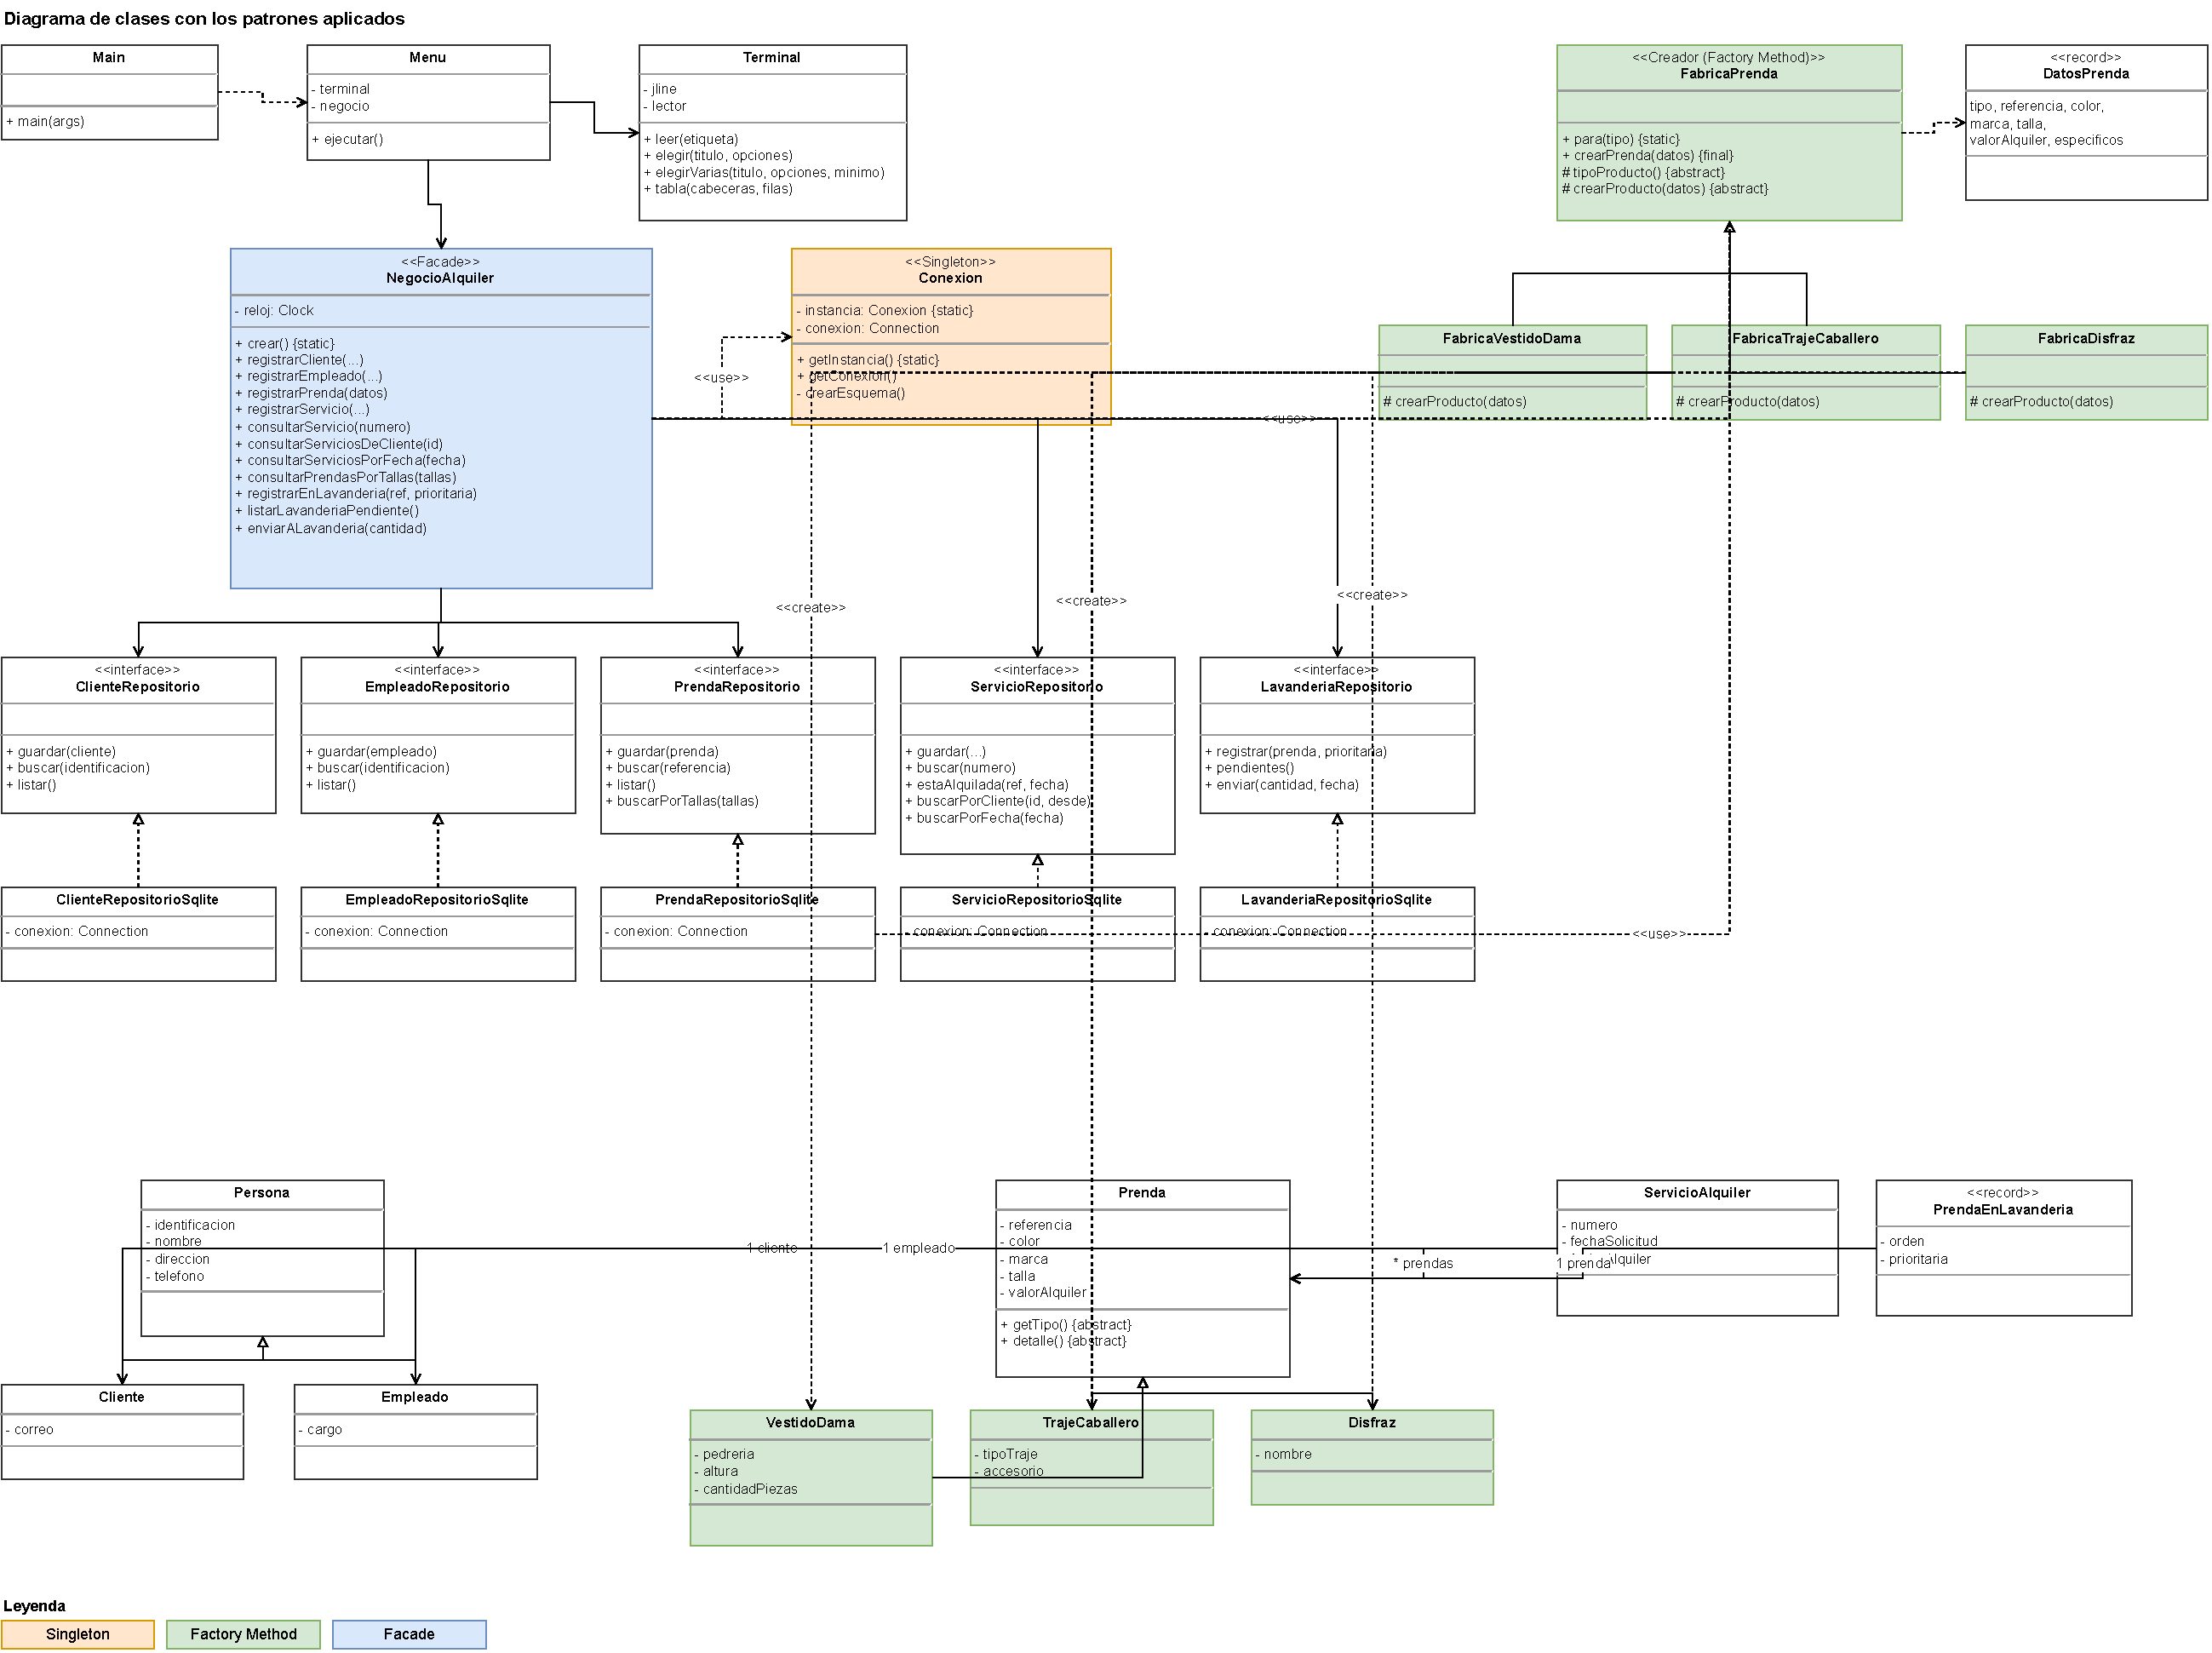
\includegraphics[width=\linewidth, height=0.82\textheight, keepaspectratio]{figures/diagrams/diagrama-clases-patrones.pdf}
\end{apafigure}
\end{landscape}

La consola gana una jerarquía de comandos y pierde las 14 operaciones que tenía \code{Menu}. El negocio gana \code{DespachoLavanderia}, que se lleva de la fachada todo lo que toca la lavandería. El modelo gana \code{ColaLavanderia} y su iterador, y \code{LavanderiaRepositorio} cambia dos de sus métodos para entregar y recibir esa cola. Las fábricas, la conexión única y el resto de los repositorios quedan como estaban.

\subsection{Command}

\code{Comando} es la interfaz del patrón, con dos métodos, \code{titulo()} para el texto de la opción y \code{ejecutar()} para la operación. La clase abstracta \code{ComandoConsola} guarda lo que todos los comandos comparten, que son los dos receptores, \code{Terminal} para leer y mostrar, y \code{NegocioAlquiler} para aplicar las reglas. Hay un comando concreto por operación, 14 en total, y cada uno contiene exactamente lo que hoy hace el método privado equivalente del menú. Las fichas y tablas que varios comandos repiten pasan a \code{Vistas}, para no duplicarlas.

\code{Menu} queda como invocador. Recibe los comandos agrupados en \code{GrupoComandos}, muestra sus títulos, ejecuta el elegido y maneja sus errores de una sola manera para todos. \code{CatalogoComandos} cumple el papel de cliente, porque crea los comandos con sus receptores y arma los grupos al iniciar la aplicación.

La \infig{fig:secuencia-command} recorre el registro de un servicio de alquiler. Quien usa la aplicación elige la opción (1) y el menú llama \code{ejecutar()} sin saber qué operación es (2). El comando concreto lee los datos con la terminal y le entrega la operación a la fachada (3), y si la fachada la rechaza con una \code{AtuendosException}, es el invocador el que muestra el error (4), igual que con cualquier otro comando.

\begin{apafigure}{secuencia-command}{Diagrama de secuencia del patrón Command en el registro de un servicio de alquiler}
\includegraphics[width=\linewidth]{figures/diagrams/diagrama-secuencia-command.pdf}
\end{apafigure}

\subsection{Iterator}

\code{ColaLavanderia} es la colección concreta. Por dentro guarda dos listas, \code{prioritarias} y \code{porLlegada}, y su método \code{agregar} pone cada registro en la que le corresponde. Implementa \code{Iterable<PrendaEnLavanderia>} de Java, que cumple el papel de colección iterable, y su método \code{iterator()} entrega un \code{IteradorLavanderia}, el iterador concreto, que implementa \code{Iterator} y recorre primero las prioritarias y después las demás. El iterador es una clase interna y privada de la cola, de modo que nadie fuera de ella conoce las dos listas.

Con esto la regla de la lavandería sale de la consulta SQL. \code{LavanderiaRepositorio} devuelve las filas pendientes por orden de llegada dentro de una \code{ColaLavanderia}, y su método \code{enviar(cantidad, fecha)} se reemplaza por \code{marcarEnviadas(registros, fecha)}, que solo guarda lo que el negocio ya decidió enviar.

La \infig{fig:secuencia-iterator} muestra el envío de una tanda. El despacho pide las pendientes (1) y el repositorio arma la cola, registro por registro. Después el despacho le pide el iterador a la cola (2) y lo recorre mientras queden prendas y no se complete la cantidad del día (3), sin saber que hay dos listas. Al final le pide al repositorio marcar como enviadas las prendas tomadas (4). El listado de pendientes recorre la misma cola con el mismo iterador, así que los dos caminos comparten un único orden.

\begin{apafigure}{secuencia-iterator}{Diagrama de secuencia del patrón Iterator en el envío de una tanda a lavandería}
\includegraphics[width=\linewidth]{figures/diagrams/diagrama-secuencia-iterator.pdf}
\end{apafigure}

\subsection{Observer}

\code{DespachoLavanderia} es el notificador. Guarda la lista de suscriptores, con métodos para suscribir y desuscribir, y concentra las tres operaciones de la lavandería, registrar, listar pendientes y enviar. \code{ObservadorLavanderia} es la interfaz suscriptora, con un solo método, \code{prendasEnviadas(envio)}, y \code{NotificacionEnvioConsola} es el suscriptor concreto que muestra el mensaje que pide el enunciado. La fachada conserva sus métodos de lavandería, pero ahora delega en el despacho, y agrega \code{suscribirALavanderia} para que la consola se registre sin conocer al despacho.

La \infig{fig:secuencia-observer} muestra los dos momentos del patrón. Al iniciar la aplicación, el catálogo de comandos crea la notificación y la suscribe una sola vez (1). Cuando alguien envía una tanda, el comando le pide el envío a la fachada y la fachada al despacho (2), que recorre la cola con el iterador de la \infig{fig:secuencia-iterator} y arma el \code{EnvioLavanderia}. Si el envío lleva prendas, el despacho avisa a cada suscriptor de la lista (3), y la notificación de consola imprime la fecha y la tabla de prendas. Si no hay nada que enviar, nadie recibe aviso, y el comando informa que no hay prendas pendientes (4).

\begin{landscape}
\begin{apafigure}{secuencia-observer}{Diagrama de secuencia del patrón Observer en la notificación de un envío a lavandería}
\includegraphics[width=\linewidth, height=0.82\textheight, keepaspectratio]{figures/diagrams/diagrama-secuencia-observer.pdf}
\end{apafigure}
\end{landscape}
